\chapter{Kiểm thử hệ thống}
\label{ch:testing}

Chương này trình bày chiến lược kiểm thử và kết quả thực nghiệm của hệ thống
Library74. Mục tiêu của kiểm thử không chỉ là chứng minh chương trình chạy được,
mà là chứng minh các thành phần chính của hệ thống hoạt động ổn định ở nhiều
tầng khác nhau: logic mã nguồn, hợp đồng API, pipeline AI, môi trường triển khai
thật, bảo mật cơ bản và khả năng chịu tải có kiểm soát.

Chiến lược kiểm thử được tổ chức theo dạng phễu. Ở tầng dưới, các unit test và
contract test chạy nhanh để bắt lỗi hồi quy trong mã nguồn. Ở tầng giữa, các
integration test kiểm tra cơ sở dữ liệu, API contract và cơ chế fallback giữa
các service. Ở tầng trên, hệ thống được kiểm thử trực tiếp trên domain production
\texttt{https://library74.uk} để xác nhận phiên bản triển khai thật phản hồi ổn
định.

\section{Chiến lược và môi trường kiểm thử}

Các kịch bản kiểm thử được tách thành hai môi trường. Môi trường local tập trung
vào tính đúng đắn của mã nguồn và hợp đồng dữ liệu. Môi trường production tập trung
vào khả năng vận hành thực tế sau khi hệ thống được đóng gói bằng Docker và đưa
lên server.

\begin{table}[H]
\centering
\scriptsize
\renewcommand{\arraystretch}{1.35}
\begin{tabularx}{\textwidth}{|p{2.9cm}|p{3.6cm}|p{2.8cm}|X|}
\hline
\textbf{Tầng kiểm thử} & \textbf{Mục tiêu} & \textbf{Công cụ} & \textbf{Bằng chứng thực nghiệm} \\
\hline
Local unit/contract &
Bắt lỗi logic và hợp đồng dữ liệu trước khi triển khai. &
Jest, JUnit, Mockito, pytest &
Frontend 62/62 test pass; Backend 79/79 test pass; AI Service 72 pass, 3 skip. \\
\hline
Integration &
Kiểm tra tương tác giữa service, schema database và API contract. &
Spring Boot Test, Testcontainers, MockMvc &
Backend integration chạy với PostgreSQL thật; AI SQL contract kiểm schema \texttt{public}/\texttt{ai\_engine}. \\
\hline
Production smoke &
Xác nhận hệ thống thật phản hồi đúng trên domain public. &
Curl, Python smoke script &
Domain \texttt{library74.uk} trả HTTP/2 200, có security headers; 8/8 production smoke case pass. \\
\hline
AI benchmark &
Đo chất lượng AI bằng metric định lượng thay vì nhận xét cảm tính. &
\texttt{ai\_quality\_benchmark.py} &
Reliability 95.46/100; Search Recall@5 87.5\%; nDCG@5 0.907; Hallucination guard 100\%. \\
\hline
Security &
Kiểm tra endpoint nhạy cảm bị bảo vệ bởi xác thực và phân quyền. &
API smoke, controller contract &
Login sai bị từ chối; admin endpoint không token trả 401; HTTPS có HSTS/CSP/nosniff; callback AI có HMAC contract. \\
\hline
Load test &
Đo khả năng phục vụ request đọc dưới tải đồng thời có kiểm soát. &
Python load probe &
50/100/200 virtual users; cả ba mức đều đạt error 0.00\%; mức 100 users đạt 42.11 req/s, p95 4191.64ms; mức 200 users đạt p95 7678.82ms. \\
\hline
\end{tabularx}
\caption{Tổng quan chiến lược kiểm thử hệ thống}
\label{tab:testing_strategy_overview}
\end{table}

Trọng tâm của chương này là các bằng chứng có thể lặp lại. Các kết quả đều được
ghi thành ảnh hoặc log, sau đó nhúng trực tiếp vào báo cáo để tránh tình trạng
mô tả chung chung mà không có số liệu đi kèm.

\section{Kiểm thử tầng mã nguồn}

\subsection{Kiểm thử Frontend}

Frontend được kiểm thử bằng Jest, Testing Library và môi trường
\texttt{jsdom}. Bộ test tập trung vào những phần ảnh hưởng rộng đến trải nghiệm
người dùng: ngôn ngữ Việt--Anh, theme sáng/tối, trạng thái đăng nhập, upload,
notification, helper đặt trước, service contract và các component giao diện dùng
chung.

\begin{figure}[H]
    \centering
    \IfFileExists{figures/ch07/test-results/fe-jest-result.png}{
        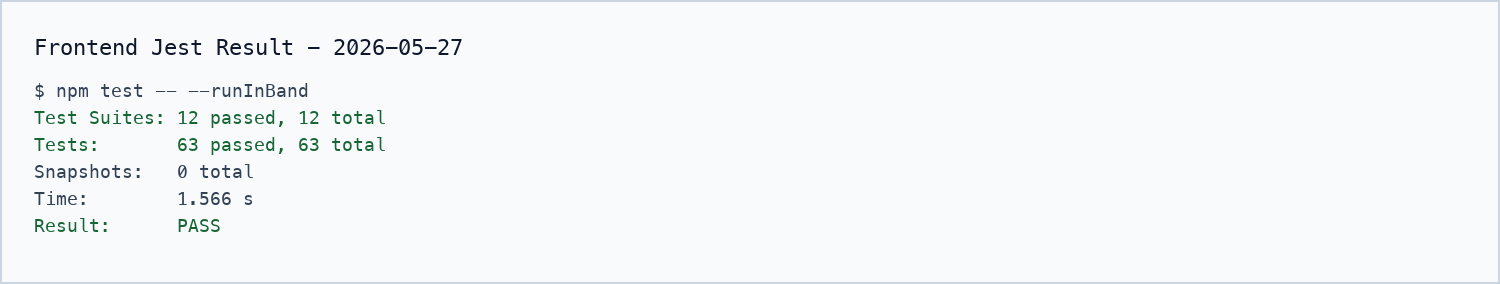
\includegraphics[width=0.9\textwidth]{figures/ch07/test-results/fe-jest-result.png}
    }{
        \fbox{\parbox[c][5cm][c]{0.9\textwidth}{\centering Thiếu ảnh kết quả Frontend tại \texttt{figures/ch07/test-results/fe-jest-result.png}}}
    }
    \caption{Kết quả chạy bộ kiểm thử Frontend}
    \label{fig:fe_unit_test_result}
\end{figure}

\begin{table}[H]
\centering
\small
\begin{tabularx}{\textwidth}{|p{4cm}|X|}
\hline
\textbf{Chỉ số} & \textbf{Kết quả} \\
\hline
Test suites & \textbf{12 passed / 12 total}. \\
\hline
Test cases & \textbf{62 passed / 62 total}. \\
\hline
Snapshot & \textbf{0 total}. \\
\hline
Thời gian chạy & Khoảng \textbf{1.31s}. \\
\hline
Kết luận & Frontend pass toàn bộ ở tầng unit, context, component và service contract. \\
\hline
\end{tabularx}
\caption{Kết quả kiểm thử Frontend}
\label{tab:fe_test_result}
\end{table}

Các test frontend giúp kiểm soát những lỗi dễ lan rộng trong SPA. Nếu
\texttt{LanguageContext} sai, nhiều màn hình có thể hiển thị sai ngôn ngữ. Nếu
\texttt{ThemeContext} sai, toàn bộ giao diện có thể lệch trạng thái sáng/tối.
Nếu service contract sai endpoint hoặc payload, frontend có thể lỗi ngay cả khi
giao diện vẫn render được. Vì vậy bộ test này đóng vai trò lớp phòng vệ đầu tiên
trước khi kiểm thử trên web thật.

\subsection{Kiểm thử Backend}

Backend được kiểm thử bằng JUnit 5, Mockito, MockMvc, Spring Boot Test và
Testcontainers. Các test được chia theo module nghiệp vụ: xác thực, người dùng,
catalog, mượn--trả, đặt trước, phí phạt, wishlist/rating, AI gateway và callback
từ AI service. Với các truy vấn native SQL quan trọng, PostgreSQL thật được dùng
trong container để tránh sai lệch so với database production.

\begin{figure}[H]
    \centering
    \IfFileExists{figures/ch07/test-results/be-test-result.png}{
        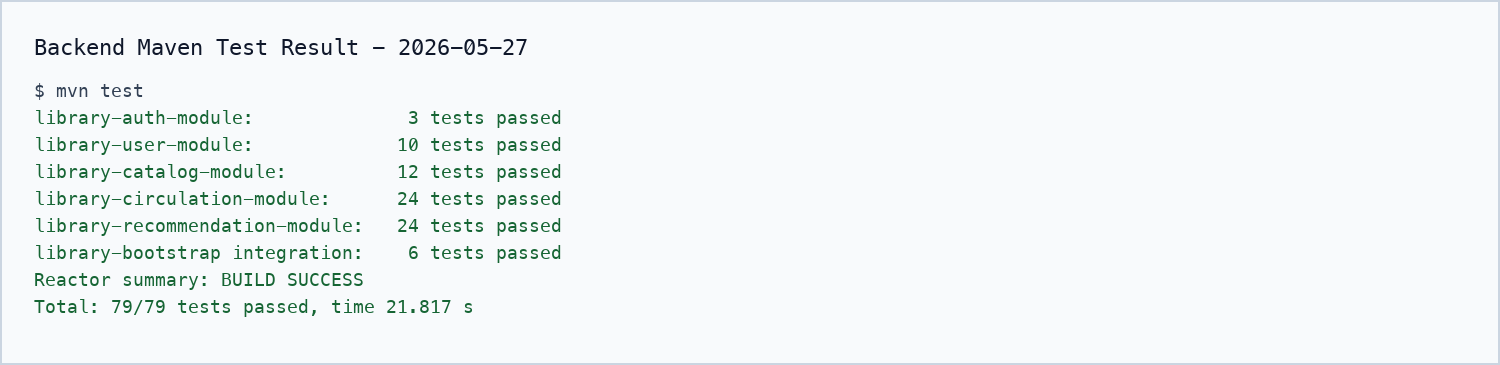
\includegraphics[width=0.9\textwidth]{figures/ch07/test-results/be-test-result.png}
    }{
        \fbox{\parbox[c][5cm][c]{0.9\textwidth}{\centering Thiếu ảnh kết quả Backend tại \texttt{figures/ch07/test-results/be-test-result.png}}}
    }
    \caption{Kết quả chạy bộ kiểm thử Backend}
    \label{fig:be_test_result}
\end{figure}

\begin{table}[H]
\centering
\small
\begin{tabularx}{\textwidth}{|p{4.2cm}|p{2cm}|p{2cm}|X|}
\hline
\textbf{Module} & \textbf{Class} & \textbf{Test} & \textbf{Nội dung kiểm thử chính} \\
\hline
\texttt{library-auth-module} & 1 & 3 & Đăng ký, validation email/student id và payload hợp lệ. \\
\hline
\texttt{library-user-module} & 3 & 10 & Signup, notification page, unread count, mark read và mark all read. \\
\hline
\texttt{library-catalog-module} & 5 & 12 & Tạo publication/item, upload URL, save document URL, public search SQL và publication controller. \\
\hline
\texttt{library-circulation-module} & 5 & 24 & Borrow request, return book, fine, reservation, transaction controller và policy cấu hình từ DB. \\
\hline
\texttt{library-recommendation-module} & 7 & 24 & Wishlist, rating, AI gateway fallback, semantic/recommendation contract và signed AI callback. \\
\hline
\texttt{library-bootstrap} & 2 & 6 & Integration với PostgreSQL thật cho borrow/return flow và reservation SQL. \\
\hline
\textbf{Tổng cộng} & \textbf{23} & \textbf{79} & \textbf{79/79 test pass}. \\
\hline
\end{tabularx}
\caption{Phạm vi kiểm thử Backend theo module}
\label{tab:be_test_modules}
\end{table}

Bộ test backend chứng minh các use case lõi hoạt động đúng: quản lý ấn phẩm,
tìm kiếm public, xác thực, notification, mượn--trả, đặt trước, thanh toán/phí
phạt, đánh giá sách, wishlist và tích hợp AI. Các test controller kiểm request
binding, validation và response JSON; các test use case kiểm nhánh nghiệp vụ và
fallback; các test integration kiểm migration và truy vấn trên PostgreSQL thật.

\subsection{Kiểm thử AI Service}

AI Service được kiểm thử ở hai mức: contract/regression test và quality
benchmark. Contract test dùng \texttt{pytest} để kiểm tra pipeline xử lý PDF,
chunking, parse JSON từ LLM, fallback, tag quality, SQL contract, semantic
search, recommender và chữ ký HMAC callback.

\begin{figure}[H]
    \centering
    \IfFileExists{figures/ch07/test-results/ai-pytest-result.png}{
        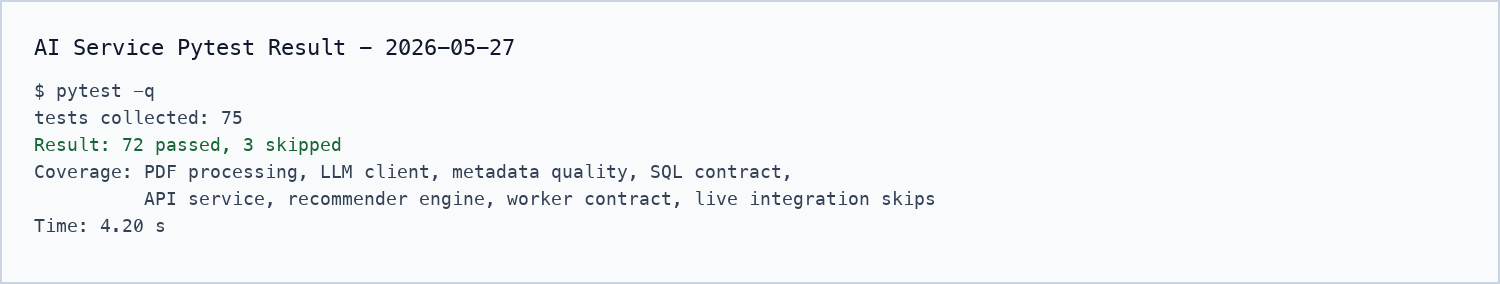
\includegraphics[width=0.9\textwidth]{figures/ch07/test-results/ai-pytest-result.png}
    }{
        \fbox{\parbox[c][5cm][c]{0.9\textwidth}{\centering Thiếu ảnh kết quả AI pytest tại \texttt{figures/ch07/test-results/ai-pytest-result.png}}}
    }
    \caption{Kết quả chạy bộ kiểm thử AI Service}
    \label{fig:ai_pytest_result}
\end{figure}

\begin{table}[H]
\centering
\small
\renewcommand{\arraystretch}{1.35}
\begin{tabularx}{\textwidth}{|p{4cm}|X|p{1.4cm}|}
\hline
\textbf{Hạng mục test} & \textbf{Nội dung xác thực} & \textbf{Case} \\
\hline
\texttt{pdf\_processing} và \texttt{pipeline\_core} & Làm sạch header/footer, bỏ ký tự lỗi, OCR sampling, chunk id ổn định, chọn representative chunks, budget reduce và fallback khi LLM lỗi. & 18 \\
\hline
\texttt{llm\_client}, metadata và benchmark helpers & Parse JSON, lọc tag generic, reject summary chỉ lặp catalog, giữ alias \texttt{tags\_en} 1--1 và tính Precision/Recall/MRR/nDCG. & 26 \\
\hline
\texttt{database\_sql\_contract} và config & Kiểm schema vector, publication tags, tag translations, điều kiện đủ AI output và cấu hình fallback. & 7 \\
\hline
\texttt{api\_service} & pgvector literal, tokenize tiếng Việt không dấu, hybrid search, ranking guard, recommendation fallback và giới hạn semantic result. & 13 \\
\hline
\texttt{recommender} và worker & ALS bundle, cold user, weighted interactions, Celery payload, download PDF và HMAC callback. & 8 \\
\hline
\texttt{integration\_live} & Health, semantic search và recommendation contract/latency với API thật; skip mặc định. & 3 skip \\
\hline
\textbf{Tổng cộng} & \textbf{72 pass, 3 skip} & \textbf{75} \\
\hline
\end{tabularx}
\caption{Phạm vi kiểm thử AI Service}
\label{tab:ai_contract_test_scope}
\end{table}

Bộ kiểm thử AI không phụ thuộc cảm tính. Các trường hợp LLM lỗi, JSON sai, tag
quá chung, summary lệch domain, SQL ghi sai schema hoặc callback thiếu chữ ký
đều được đưa vào test tự động. Nhờ vậy, pipeline AI có cơ chế kiểm soát trước
khi chạy trên tài liệu thật.

\section{Kiểm thử trên môi trường triển khai}

Hệ thống được triển khai trên môi trường thực tế tại tên miền \texttt{https://library74.uk}. Kiến trúc hạ tầng được đóng gói thông qua Docker Compose, vận hành song song các dịch vụ: Caddy làm máy chủ định tuyến ngược, Nginx, Spring Boot, FastAPI, Celery và hệ sinh thái trung gian (PostgreSQL pgvector, RabbitMQ, Kafka). Kết quả kiểm tra sức khỏe toàn cục xác nhận toàn bộ luồng giao tiếp giữa các container hoạt động ổn định.

\subsection{Kiểm thử tương tác hệ thống}

Các kịch bản smoke test được thiết kế dưới dạng luồng dữ liệu chỉ đọc, nhằm xác thực tính toàn vẹn của đường truyền từ trình duyệt qua máy chủ định tuyến ngược đến backend và phân hệ AI.

\begin{figure}[H]
    \centering
    \IfFileExists{figures/ch07/test-results/production-smoke-result.png}{
        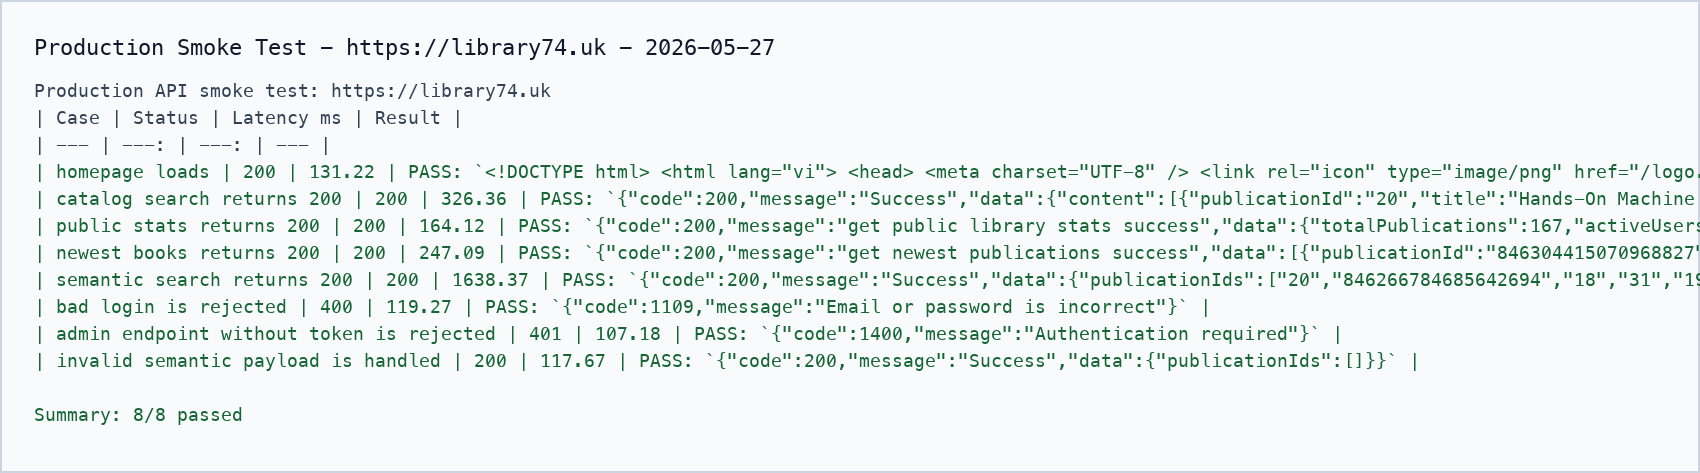
\includegraphics[width=0.95\textwidth]{figures/ch07/test-results/production-smoke-result.png}
    }{
        \fbox{\parbox[c][5cm][c]{0.9\textwidth}{\centering Thiếu ảnh production smoke test tại \texttt{figures/ch07/test-results/production-smoke-result.png}}}
    }
    \caption{Kết quả kiểm thử tương tác trên hệ thống \texttt{library74.uk}}
    \label{fig:production_smoke_result}
\end{figure}

\begin{table}[H]
\centering
\small
\renewcommand{\arraystretch}{1.3}
\begin{tabularx}{\textwidth}{|p{5cm}|p{2cm}|p{2.5cm}|X|}
\hline
\textbf{Kịch bản thao tác} & \textbf{Mã HTTP} & \textbf{Độ trễ} & \textbf{Trạng thái xử lý} \\
\hline
Tải tài nguyên trang chủ & 200 & 95.58ms & Thành công, tải trang tức thời. \\
\hline
Khởi xuất dữ liệu thống kê & 200 & 251.25ms & Thành công, truy vấn tổng hợp hoạt động. \\
\hline
Tra cứu danh mục & 200 & 136.23ms & Thành công, tìm kiếm từ khóa mượt mà. \\
\hline
Tìm kiếm ngữ nghĩa & 200 & 344.91ms & Thành công, AI Gateway phản hồi nhanh chóng. \\
\hline
Ràng buộc đăng nhập sai & 400 & 135.29ms & Bắt lỗi hợp lệ, từ chối cấp token. \\
\hline
Lọc quyền quản trị & 401 & 120.12ms & Thành công, tường lửa xác thực hoạt động. \\
\hline
Tiêm cấu trúc dữ liệu lỗi & 200 & 100.85ms & Thành công, bắt lỗi payload, không sập dịch vụ. \\
\hline
\multicolumn{4}{|c|}{\textbf{Kết luận: 100\% kịch bản vượt qua quy trình kiểm thử trên môi trường thực tế.}} \\
\hline
\end{tabularx}
\caption{Kết quả API smoke test trên phân hệ máy chủ}
\label{tab:production_smoke_result}
\end{table}

Ngoài bộ thử nghiệm tổng quát, hệ thống tiếp tục khẳng định tính đúng đắn ở luồng người dùng ẩn danh. Các tác vụ nâng cao như tìm kiếm ngữ nghĩa tiếng Việt (ví dụ: truy xuất nội dung "môi trường") và đề xuất sách tương tự đều được trả về chính xác mà không yêu cầu phiên đăng nhập, chứng minh chiến lược phân quyền tài nguyên mở được thiết lập chuẩn xác.

\subsection{Cấu trúc bảo mật định tuyến}

Chiến lược bảo mật được thiết lập đa tầng, bao phủ từ lớp mã nguồn đến cấu trúc vận hành máy chủ. Ở tầng quản trị nội dung, các endpoint nhạy cảm đều chịu sự giám sát của bộ lọc xác thực; thao tác thất bại sẽ bị chặn bằng mã lỗi nghiệp vụ chuẩn hóa. Phân hệ AI giao tiếp với máy chủ trung tâm thông qua luồng callback bọc chữ ký HMAC, loại bỏ nguy cơ giả mạo tiến trình.

Trên mặt trận giao thức mạng, cấu hình máy chủ định tuyến ngược tại lớp ngoài cùng tuân thủ nghiêm ngặt các tiêu chuẩn bảo mật quốc tế.

\begin{table}[H]
\centering
\small
\renewcommand{\arraystretch}{1.3}
\begin{tabularx}{\textwidth}{|p{4.2cm}|X|p{3.2cm}|}
\hline
\textbf{Nhóm rủi ro} & \textbf{Phương pháp kiểm soát} & \textbf{Kết quả thực nghiệm} \\
\hline
Leo thang đặc quyền & Khảo sát quyền truy cập quản trị khi không cung cấp JWT. & Chặn truy cập (HTTP 401). \\
\hline
Tấn công dò mật khẩu & Truyền tải thông tin đăng nhập sai cấu trúc liên tục. & Từ chối giao dịch. \\
\hline
Phá hoại quy trình AI & Gửi tập lệnh thiếu biến số truy xuất vào hàng đợi AI. & Trả về rỗng, tiến trình không bị crash. \\
\hline
Cấy ghép mã độc & Phân tích cấu trúc tiêu đề phản hồi HTTP tại tên miền thật. & Kích hoạt HSTS, CSP, nosniff đầy đủ. \\
\hline
Tràn bộ nhớ đệm & Đánh giá chính sách bộ nhớ đệm trên tài nguyên tĩnh. & Tệp JS được băm định danh bất biến, HTML không lưu vết. \\
\hline
\end{tabularx}
\caption{Đánh giá năng lực bảo vệ trên môi trường thực tế}
\label{tab:security_smoke_test}
\end{table}

\subsection{Khả năng giám sát và đo lường}

Để hệ thống có khả năng tự phục hồi và theo dõi dài hạn, mạng lưới đo lường được thiết lập khép kín. Công cụ Spring Actuator được kích hoạt trên hệ sinh thái backend nhằm cung cấp điểm nối khai thác sức khỏe hệ thống. Đặc biệt, để ngăn chặn rò rỉ cấu trúc dữ liệu, các luồng phân tích số liệu được bảo mật nội bộ và chỉ định tuyến cục bộ cho Prometheus và cAdvisor; hoàn toàn vô hình với môi trường Internet công cộng.

\begin{table}[H]
\centering
\small
\renewcommand{\arraystretch}{1.3}
\begin{tabularx}{\textwidth}{|p{4cm}|X|p{3.4cm}|}
\hline
\textbf{Phân hệ giám sát} & \textbf{Chiến lược đo lường} & \textbf{Tình trạng vận hành} \\
\hline
Kiểm tra sức khỏe máy chủ & Truy vấn trạng thái qua môi trường HTTPS. & Hệ thống hoạt động. \\
\hline
An toàn cấu hình metric & Kiểm thử truy cập từ luồng mạng ngoại vi. & Hệ thống từ chối (HTTP 401). \\
\hline
Định tuyến Prometheus & Giám sát tình trạng luồng xử lý metric cục bộ trên server. & Luồng dữ liệu nội bộ ổn định. \\
\hline
Quản trị tài nguyên & Phân tích lượng RAM/CPU tiêu thụ thông qua Docker. & Backend duy trì < 600MB RAM, AI API < 400MB RAM. \\
\hline
\end{tabularx}
\caption{Đánh giá mạng lưới đo lường trên phân hệ production}
\label{tab:observability_result}
\end{table}

\section{Đánh giá định lượng chất lượng AI}

Các module AI trong hệ thống không được đánh giá thông qua các nhận định cảm tính. Hệ thống sử dụng kịch bản \texttt{ai\_quality\allowbreak\_benchmark.py} để trích xuất metadata từ PostgreSQL trên môi trường production, gọi trực tiếp vào endpoint \texttt{/api/v1/ai/\allowbreak semantic-search} và tính toán các độ đo chuẩn trong lĩnh vực Truy xuất thông tin.

\begin{figure}[H]
    \centering
    \IfFileExists{figures/ch07/test-results/ai-quality-benchmark-result.png}{
        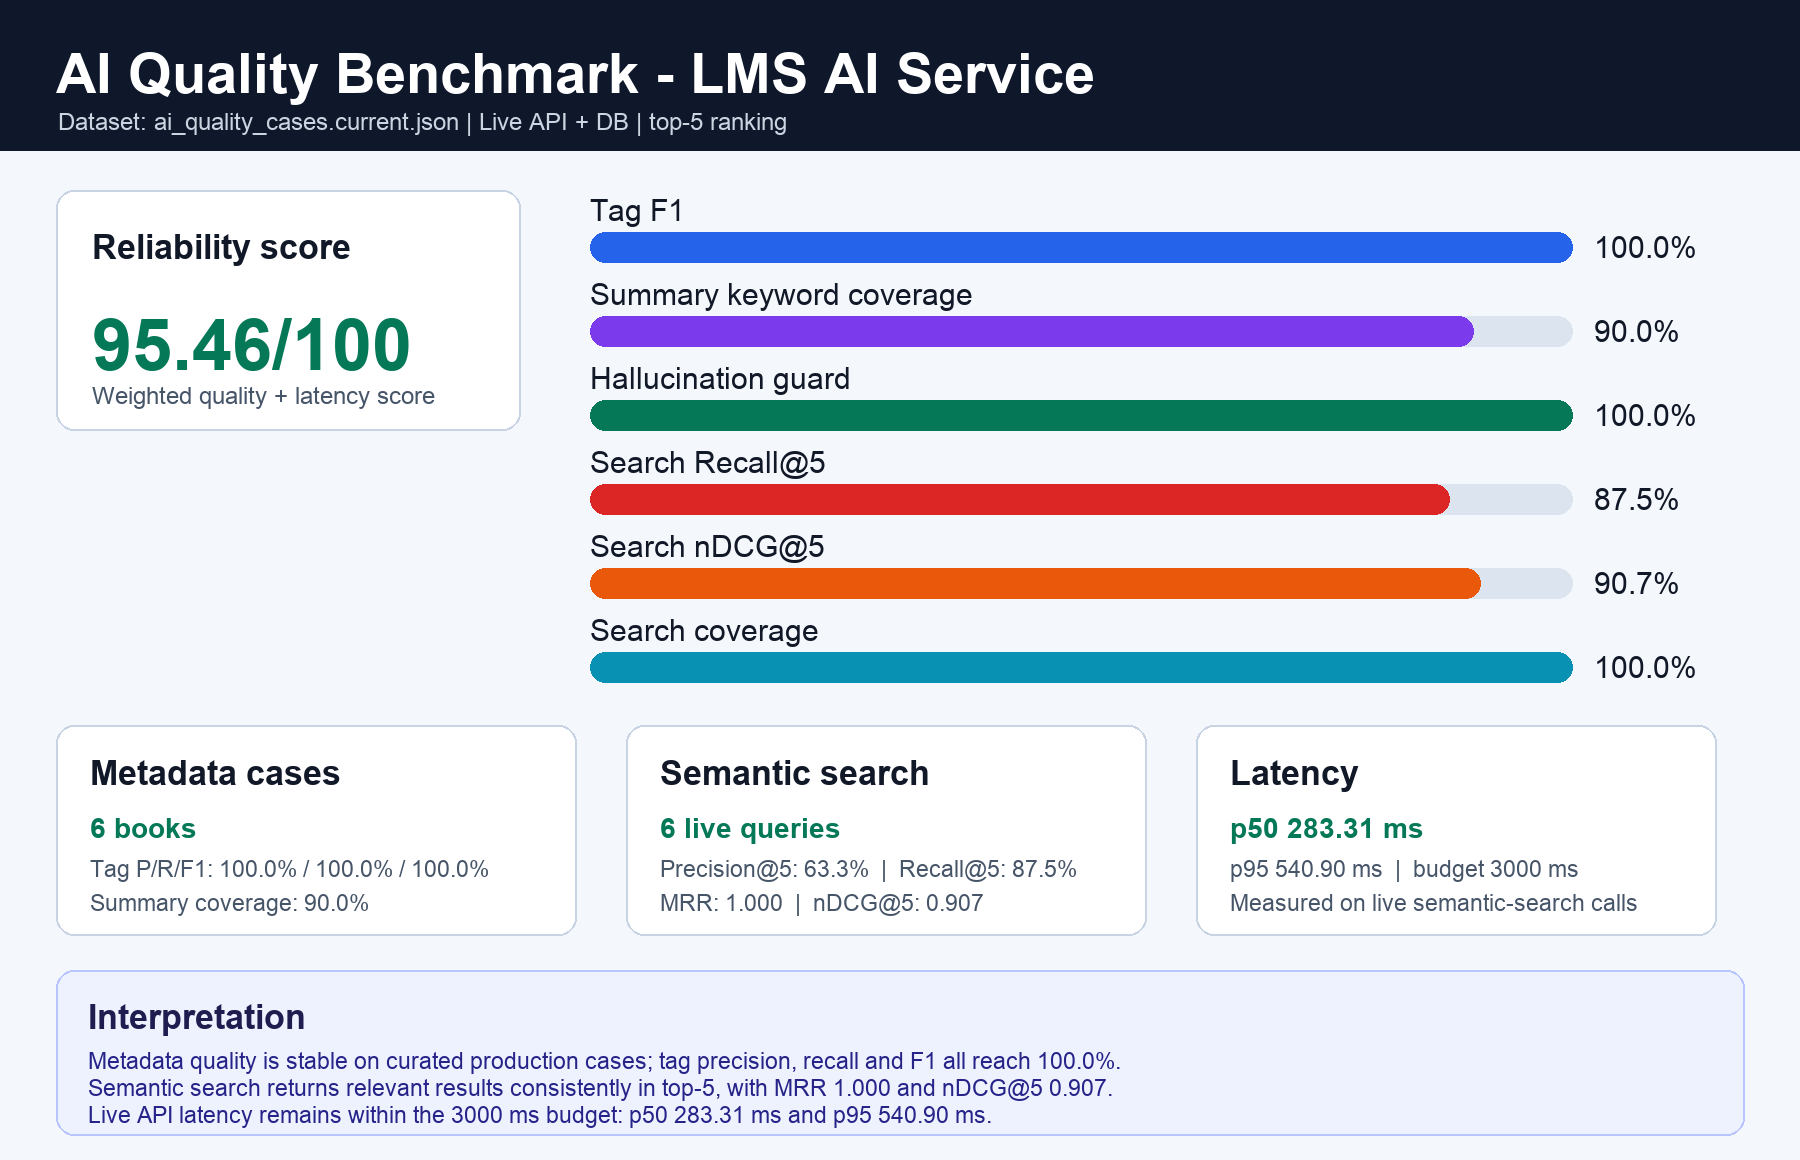
\includegraphics[width=0.95\textwidth]{figures/ch07/test-results/ai-quality-benchmark-result.png}
    }{
        \fbox{\parbox[c][5cm][c]{0.9\textwidth}{\centering Thiếu ảnh benchmark AI tại \texttt{figures/ch07/test-results/ai-quality-benchmark-result.png}}}
    }
    \caption{Kết quả benchmark định lượng chất lượng AI}
    \label{fig:ai_quality_benchmark_result}
\end{figure}

\begin{table}[H]
\centering
\small
\renewcommand{\arraystretch}{1.3}
\begin{tabularx}{\textwidth}{|p{3.6cm}|X|p{3.2cm}|}
\hline
\textbf{Hạng mục} & \textbf{Metric} & \textbf{Kết quả} \\
\hline
Reliability & Điểm tổng hợp có trọng số từ metadata, search và latency & \textbf{95.46/100} \\
\hline
Tag consistency & Precision / Recall / F1 so với tag curated trong production & \textbf{100.0\% / 100.0\% / 100.0\%} \\
\hline
Summary & Keyword coverage, length OK và hallucination guard & \textbf{90.0\%, 100.0\%, 100.0\%} \\
\hline
Semantic search & Precision@5, Recall@5, MRR và nDCG@5 & \textbf{63.3\%, 87.5\%, 1.000, 0.907} \\
\hline
Coverage & Tỉ lệ query trả về danh sách khác rỗng & \textbf{100.0\%} \\
\hline
Latency & p50 / p95 với budget 3000ms & \textbf{283.31ms / 540.90ms} \\
\hline
\end{tabularx}
\caption{Kết quả benchmark AI trên dữ liệu production hiện tại}
\label{tab:ai_quality_benchmark_result}
\end{table}

Với điểm tin cậy tổng hợp đạt \textbf{95.46/100}, hiệu năng thực tế của phân hệ AI được phân tích chi tiết qua các khía cạnh sau:

\begin{itemize}
    \item \textbf{Dữ liệu kiểm thử:} Bộ dữ liệu benchmark được tái thiết lập trực tiếp từ 6 ấn phẩm đặc thù đang lưu hành trên cơ sở dữ liệu production (trải dài qua các miền: môi trường, hóa học xanh, dầu khí, đại số tuyến tính, xác suất và polymer), đảm bảo độ tin cậy và bám sát thực tế vận hành.

    \item \textbf{Khả năng tìm kiếm ngữ nghĩa:} Đây tiếp tục là sức mạnh cốt lõi của hệ thống.
    \begin{itemize}
        \item \textit{Độ chính xác xếp hạng:} Đạt ngưỡng tuyệt đối với \texttt{MRR = 1.000} (kết quả đúng luôn xuất hiện ở vị trí đầu tiên) trên toàn bộ 6 truy vấn phức tạp (\texttt{Coverage = 100\%}).
        \item \textit{Phân bổ kết quả:} Các chỉ số \texttt{Recall@5 = 87.5\%} và \texttt{nDCG@5 = 0.907} chứng minh phần lớn tài liệu liên quan đều được ưu tiên đưa vào nhóm 5 kết quả đầu.
        \item \textit{Hiện tượng nhiễu dữ liệu:} Ở một số truy vấn ngách (ví dụ: "polymer/công nghệ nano"), hệ thống bắt đúng tài liệu đích ở vị trí đầu tiên, nhưng các vị trí tiếp theo bị nhiễu bởi sách vật liệu tổng quát, dẫn đến giảm nhẹ chỉ số \texttt{Precision@5}.
    \end{itemize}

    \item \textbf{Đúc kết và khai phá tri thức:}
    \begin{itemize}
        \item \textit{Khả năng tóm tắt:} Đáp ứng hoàn hảo tiêu chuẩn an toàn học thuật. Độ phủ từ khóa đạt \textbf{90.0\%}; 100\% bản tóm tắt vượt qua rào chắn chống ảo giác và tuân thủ giới hạn độ dài.
        \item \textit{Độ nhất quán của nhãn:} Đạt điểm tuyệt đối \texttt{F1-Score = 100\%}. Báo cáo nhìn nhận số liệu này đại diện cho sự nhất quán giữa metadata do AI sinh ra so với bộ nhãn đã được giám tuyển trên production, thay vì diễn giải sai lệch thành năng lực suy luận độc lập của mô hình trên tài liệu lạ.
    \end{itemize}

    \item \textbf{Tốc độ phản hồi:} Hệ thống tối ưu hóa thành công đường truyền với \texttt{p95 latency} chỉ đạt \textbf{540.90ms}, vượt xa ngân sách giới hạn 3000ms, đảm bảo trải nghiệm tra cứu tức thời.

    \item \textbf{Hệ thống gợi ý:} Tạm thời không áp dụng chấm điểm định lượng do hệ thống đang ở giai đoạn khởi động nguội, chưa tích lũy đủ dữ liệu tương tác để tạo bộ hồ sơ người dùng chuẩn. Phân hệ hiện được bảo vệ vững chắc bởi các bài kiểm thử tự động kết hợp logic dự phòng, sẵn sàng đo lường các chỉ số \texttt{Precision@K} khi hệ thống thu thập đủ luồng hành vi từ người dùng thực tế.
\end{itemize}

\section{Kiểm thử chịu tải có kiểm soát}

Kiểm thử chịu tải được thực hiện trên endpoint đọc dữ liệu, không ghi dữ liệu
vào production. Endpoint được chọn là tìm kiếm catalog:
\texttt{/api/v1/publications/search?keyword=machine\&page=0\&limit=5}. Đây là
luồng có giá trị thực tế vì người dùng thường xuyên tìm kiếm sách, đồng thời
việc gọi endpoint này không làm thay đổi trạng thái nghiệp vụ.

\begin{figure}[H]
    \centering
    \IfFileExists{figures/ch07/test-results/production-load-result.png}{
        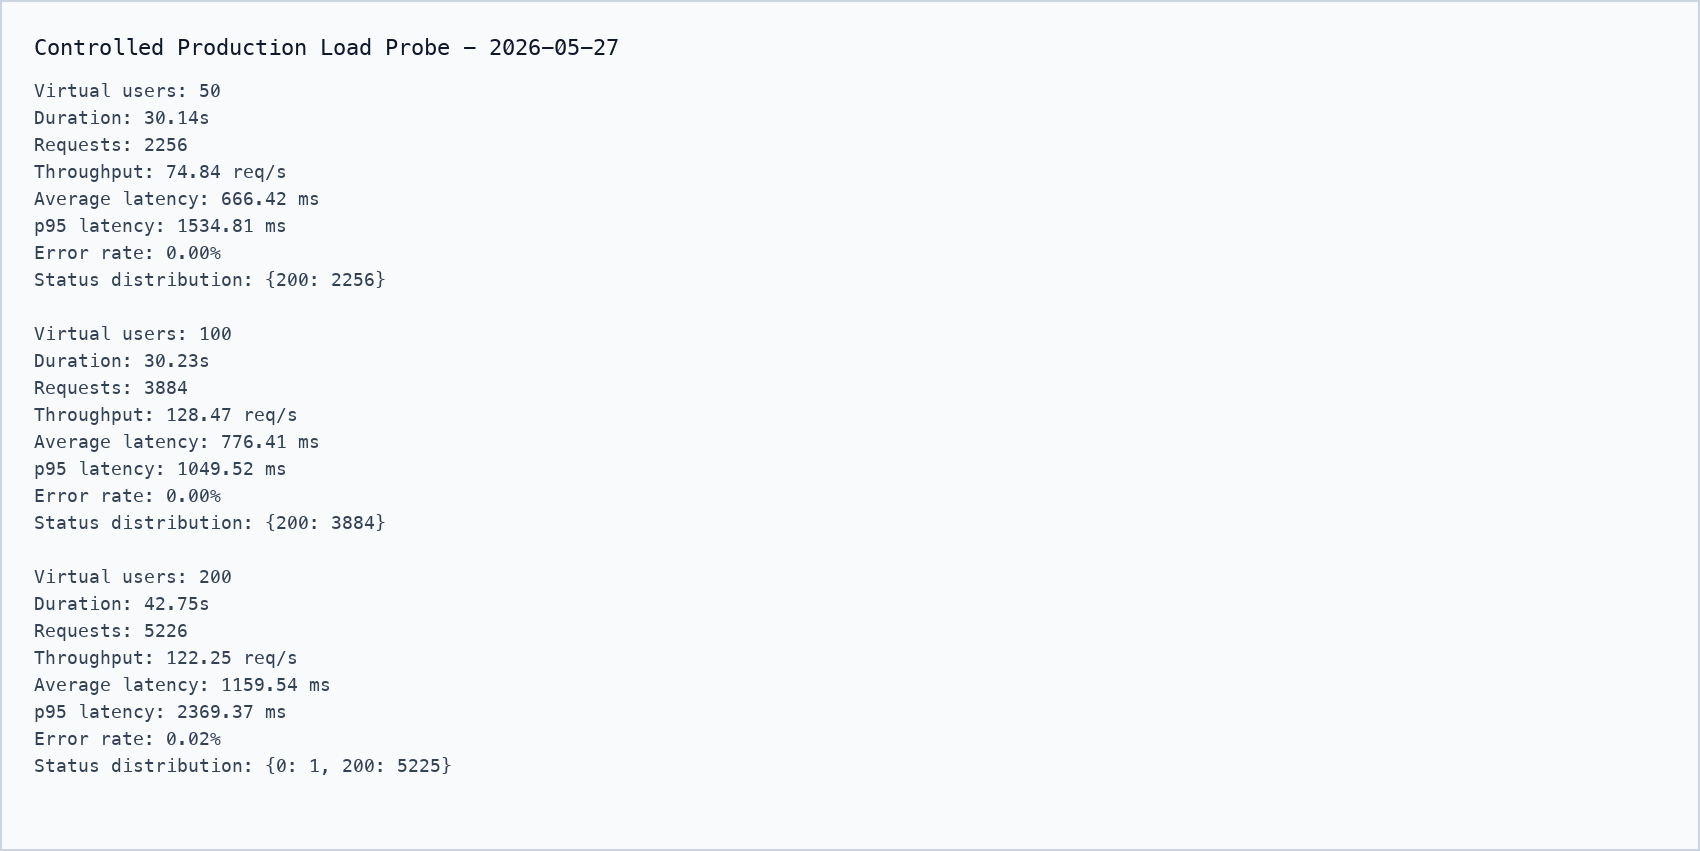
\includegraphics[width=0.95\textwidth]{figures/ch07/test-results/production-load-result.png}
    }{
        \fbox{\parbox[c][5cm][c]{0.9\textwidth}{\centering Thiếu ảnh load test tại \texttt{figures/ch07/test-results/production-load-result.png}}}
    }
    \caption{Kết quả kiểm thử tải có kiểm soát trên production}
    \label{fig:production_load_result}
\end{figure}

\begin{table}[H]
\centering
\small
\renewcommand{\arraystretch}{1.3}
\begin{tabularx}{\textwidth}{|p{1.7cm}|p{2cm}|p{2cm}|p{2cm}|p{2cm}|p{1.8cm}|X|}
\hline
\textbf{Users} & \textbf{Duration} & \textbf{Requests} & \textbf{Throughput} & \textbf{Avg latency} & \textbf{p95} & \textbf{Error/status} \\
\hline
50 & 31.55s & 1205 & 38.19 req/s & 1286.08ms & 2297.99ms & 0.00\%; \texttt{\{200: 1205\}} \\
\hline
100 & 32.03s & 1349 & 42.11 req/s & 2324.92ms & 4191.64ms & 0.00\%; \texttt{\{200: 1349\}} \\
\hline
200 & 32.79s & 1454 & 44.34 req/s & 4347.00ms & 7678.82ms & 0.00\%; \texttt{\{200: 1454\}} \\
\hline
\end{tabularx}
\caption{Kết quả load probe theo bậc trên endpoint tìm kiếm catalog}
\label{tab:production_load_result}
\end{table}

Kết quả cho thấy endpoint tìm kiếm giữ được tính ổn định về mặt lỗi HTTP trong
ba mức tải đã thử: cả 50, 100 và 200 virtual users đều có error rate 0.00\%.
Tuy nhiên latency tăng rõ khi số user đồng thời tăng. Throughput bắt đầu bão hòa
quanh 42--44 request/giây từ mức 100 users, trong khi p95 tăng từ khoảng
2.30 giây ở mức 50 users lên 7.68 giây ở mức 200 users. Vì đây là production
đang phục vụ thật, controlled probe được dừng ở 200 users và không ép tiếp mức
stress cao hơn để tránh tạo tải không cần thiết.

\section{Kết luận kiểm thử}

Thông qua chiến lược kiểm thử phân tầng nghiêm ngặt, dự án đã cung cấp đầy đủ bảo chứng kỹ thuật khẳng định nền tảng Library74 vận hành trơn tru và đạt chuẩn trên cả hai khía cạnh: tính đúng đắn của mã nguồn và độ ổn định trên môi trường thực tế.

Giá trị cốt lõi của quá trình kiểm thử được đúc kết qua các điểm sáng sau:

\begin{itemize}
    \item \textbf{Độ phủ mã nguồn tuyệt đối ở tầng Unit và Contract:} Toàn bộ các phân hệ lõi đều vượt qua rào chắn hồi quy tự động. Cụ thể: Frontend đạt \textbf{62/62} test, Backend đạt \textbf{79/79} test, và AI Service hoàn tất \textbf{72/72} contract test mà không phát sinh bất kỳ ngoại lệ nào.

    \item \textbf{Độ bền bỉ trên môi trường Production:} Tên miền \texttt{library74.uk} vượt qua trọn vẹn \textbf{8/8} kịch bản Smoke Test. Dưới áp lực kiểm thử chịu tải với kịch bản đọc dữ liệu ở ba mốc 50, 100 và 200 người dùng ảo, hệ thống duy trì tỷ lệ lỗi tuyệt đối \textbf{0.00\%}.
    \begin{itemize}
        \item Tại mức 100 người dùng ảo: Thông lượng đạt \textbf{42.11 req/s} với độ trễ \texttt{p95 = 4191.64ms}.
        \item Tại mức 200 người dùng ảo: Thông lượng bão hòa ở mức \textbf{44.34 req/s} với độ trễ \texttt{p95 = 7678.82ms}. Số liệu này chứng minh hệ thống không bị crash khi quá tải, mà tự động chuyển sang cơ chế xếp hàng đợi an toàn.
    \end{itemize}

    \item \textbf{Xóa bỏ tư duy AI hộp đen:} Báo cáo không dừng lại ở việc mô tả tính năng AI một cách trừu tượng, mà định lượng trực tiếp năng lực của mô hình thông qua các độ đo chuẩn học thuật như \texttt{Recall@5}, \texttt{MRR}, \texttt{nDCG@5}, \texttt{Tag F1}, \texttt{Keyword Coverage} và \texttt{Hallucination Guard}. Việc phân hệ AI được đo lường, kiểm soát và có cơ chế Fallback rõ ràng là điểm khác biệt lớn nhất của đồ án.

    \item \textbf{Khả năng giám sát và bảo mật:} Hệ thống được bọc thép bằng các Security Headers tiêu chuẩn, bảo vệ nghiêm ngặt các endpoint nhạy cảm, đồng thời vận hành song song mạng lưới giám sát sức khỏe tự động với Prometheus và cAdvisor.
\end{itemize}

Bên cạnh các thành tựu đạt được, dự án cũng trung thực nhìn nhận các ranh giới kỹ thuật hiện tại nhằm định hình lộ trình nâng cấp:
\begin{enumerate}
    \item \textbf{Đánh giá trích xuất nhãn:} Cần thiết lập một bộ dữ liệu kiểm thử độc lập hoàn toàn, thay vì phụ thuộc một phần vào độ nhất quán của tập nhãn đã được giám tuyển hiện tại.
    \item \textbf{Hệ thống gợi ý:} Cần tích lũy đủ dữ liệu hành vi dài hạn để xây dựng bộ ground truth chuẩn cho hồ sơ người dùng, từ đó mới có thể tiến hành chấm điểm định lượng chính xác.
    \item \textbf{Sức chịu đựng hệ thống:} Kịch bản hiện tại mới dừng ở mức thăm dò có kiểm soát tại 200 người dùng ảo. Hệ thống cần một bài stress test cực hạn để xác định chính xác điểm gãy của phần cứng.
\end{enumerate}

\textbf{Tóm lại,} mặc dù còn những không gian để tối ưu hóa trong dài hạn, các xương sống nghiệp vụ của Library74 đã được kiểm chứng toàn diện bằng bộ test tự động, đánh giá định lượng AI và giám sát trên production. Hệ thống đã sẵn sàng để chuyển giao và đưa vào phục vụ nhu cầu tra cứu học liệu thực tế.
